\documentclass[11pt]{article}

\usepackage{geometry}
\geometry{a4paper, portrait, margin=3cm}

\usepackage{todonotes}
%TC:macro \todo [ignore]

\usepackage{helvet}
\renewcommand{\familydefault}{\sfdefault}

\usepackage{setspace}
\usepackage{indentfirst}
\usepackage{siunitx}
\usepackage{amssymb}
\usepackage{parskip}
\usepackage{lineno}
\usepackage{graphicx}
\usepackage[labelfont=bf]{caption}
\usepackage{float}
\usepackage[authoryear]{natbib}
\usepackage[T1]{fontenc}
\usepackage{multirow}
\usepackage{multicol}
\usepackage{rotating}

%opening

\begin{document}

	\begin{titlepage}
		
		\begin{center}
			
		\begin{figure}[H]
		\centering
		\includegraphics[width = \textwidth]{../Data/logo.jpg}
	    \end{figure}

		
		\vspace*{3cm}
		\Huge
		\textbf{Comparison of Performance of Models Fitting Organisms in Different Habitats }\\
		
		\vspace{5cm}
		\Large
		
		\textbf{Jiqiu Wu}\\   
		\vspace*{1cm}
		\textbf{j.wu18@imperial.ac.uk}\\
		\vspace*{1cm}
		\textbf{Department of Life Sciences}\\
		\vspace*{1cm}
 
		
		\vspace{2cm}
		
		\end{center}

	\end{titlepage}
	
	\clearpage
	\tableofcontents
	
	
	\linenumbers
	\doublespacing
	\newpage
	\section*{Abstract}
Accurate prediction of the impact of climate change on metabolic rate has overwhelmingly practical siginificance. This study shows that the phenomenal model has stronger predicting ability. And much more attention and patience are supposed to pay to mechanistic models. In order to get the best prediction, scholars should choose models and model selection criteria with caution.
	
	
		
	\section{Introduction}
Metabolism theory provides a foundation for using first principles of physics, chemistry, and biology to link the performance from the molecular level\citep{allen2006kinetic} the ecology level of population\citep{savage2004effects}, community and ecosystem\citep{brown2004toward}. The theoretical basis is the core of metabolism consists of a small number of reactions that are ultimately dependent on temperature\citep{gillooly2001effects}.

Climate change is projected to have significant effects on public health\citep{woodward2014climate}, agriculture\citep{howden2007adapting}, and fishing\citep{brander2007global}. Prediction of the impacts of climate change on freshwater, marine, and terrestrial environments can assist the management of agriculture, fishery, and wildlife conservation\citep{prowse2009implications}.

Here, a large dataset called BioTraits\citep{della2013thermal}, one phenomenological models, Cubic model, one mechanistic models with three forms, Schoolfield model, Schoolfield model for low temperature, and Schoolfield model for high temperature model, three selection criteria, AIC, BIC, and AICc were used to study two main questions: (1) Is there any difference in the performance of organisms in different habitats fitted by different models? (2) If the answer of Question (1) is YES, so what is the best model in different habitats?

In this study, the results show: (1) The differences in performances exist; (2) In most cases, phenomenological model fits much better than mechanistic models. By different model selection, the best mechanistic model varies under different environments. Consequently, researchers should choose the most appropriate model selection criteria according to the habitat where the research organism live in, the size of sample, and the number of parameters, and choose the best model cautiously.
		
\section{Methods}
\subsection{Data}
BioTraits\citep{della2013thermal} that consists of 25826 rows of data from 2165 researches from small scale, like photosynthesis rate and respiration rate to large scale, like population growth rate. The habitats included marine, terrestrial, and freshwater environments. At kingdom level, the organisms were composed of archaea, bacteria, chromista, metazoa, fungi, plantae, and protista. 

But a large number of low quality data exist, NA, zero, and negetive value. If the body temperature of consumer were missing, and ambient temperature replaced. Besides, the researches with less than 8 data points were filtered out.

\subsection{Start values calculating for Schoolfield model}
Before fitting School model to the dataset, the starting value of the parameters were calculated. First, the optimal temperature at which the trait value is highest. Before and after this optimal temperature, linear regression analysis were conducted twice respectively. 

$E$ is the slope for the part after the optimal temperature, and its biological interpretation is the activation energy. $E_h$ is the slope before the optical temperature, and the biological interpretation is the de-activation energy of enzyme at high temperature. $T_h$ is the at which the enzyme is 50\% high-temperature deactivated, and was determined as the mean value of the maximal and optical temperature. $E_l$ is the slope for the part before the optimal temperature, and the biological interpretation is the de-activation energy of enzyme at low temperature. $T_l$ is the at which the enzyme is 50\% low-temperature deactivated, and was determined as the mean value of the minimal and optical temperature. Schoofield model would be discussed further in the following models section.

\subsection{Models}
\subsubsection{Phenomenological model}
Generally, the thermal performance curves have unimodal shape. Cubic model\citep{callaway1959model} are often used to study.  This is Cubic model:
\begin{equation}
B = B_O + B_1 * T + B_2 * T^2 + B_3 * T ^ 3
\end{equation}
The parameters: $B_O$, $B_1$, $B_2$, and $B_3$ don't have biological interpretations. This equation gives the trait value at the given $T$ temperature.

\subsubsection{Mechanistic models}
A biological understanding of the response of metabolic rate to temperature is critical. Consequently, Schoolfiel model is used. This is full Schoolfiel model\citep{schoolfield1981non}:

\begin{equation}
B = \frac{B_0 e^{\frac{-E}{k}(\frac{1}{T} - \frac{1}{283.15})}} {1 + e^{\frac{E_l} {k} (\frac{1}{T_l} - \frac{1}{T})} + e^{\frac{E_h}{k} (\frac{1}{T_h} - \frac{1}{T})}}
\end{equation}

Where k is the Boltzmann constant $(8.617 * 10^{-5} eV ⋅ K^{-1})$, $B$ the value of the trait at a given temperature $T$ (K)  (K = $^\text{o}$C + 273.15), while $B_0$ is the trait value at 283.15 K (10$^\text{o}$C) which stands for the value of the growth rate at low temperature. $E_l$ and $E_h$ are the enzyme's low-temperature de-activation energy ($eV$) and high-temperature de-activation energy ($eV$).  $T_l$ and $T_h$ are the at which the enzyme is 50\% low-temperature deactivated and 50\% high-temperature deactivated. $E$ is the activation energy ($eV$).

In some cases, low temperature inactivation and high temperature are not available, the simplified models for low temperature and high temperature are more appropriate. 
This is the Schoolfield model for low temperature:

\begin{equation}
B = \frac{B_0 e^{\frac{-E}{k}(\frac{1}{T} - \frac{1}{283.15})}} {1 + e^{\frac{E_l} {k} (\frac{1}{T_l} - \frac{1}{T})} }
\end{equation}

This is the Schoolfield model for high temperature:

\begin{equation}
B = \frac{B_0 e^{\frac{-E}{k}(\frac{1}{T} - \frac{1}{283.15})}} {1 +  e^{\frac{E_h}{k} (\frac{1}{T_h} - \frac{1}{T})}}
\end{equation}
\subsection{Model selection criteria}
Candidate models are compared to one another by evaluating the relative support in the observed data for every model\citep{johnson2004model}. Akaike information criteria (AIC)\citep{burnham2004multimodel}, Bayesian information criterion (BIC)\citep{schwarz1978estimating}, and Small sample unbiased AIC(AICC)\citep{burnham2004multimodel}.

AS for AIC criteria, after models were fitted within each research, the minimal AIC was determined, and the delta AIC was calculated. Finally, the relative weight of every model was calculated. The best model is the model with most support\citep{burnham2004multimodel}.

\subsection{Statistics analysis}
P values were calculated using Kruskal-Wallis test\citep{vargha1998kruskal} to compare the significant difference in multiple groups. In two groups, p values were calculated using Mann-Whitney test\citep{ruxton2006unequal}. The reason is that the normal distribution and consistent variance can't be guaranteed.
\subsection{Visualizaton}
The histogram suing point geom with the size of samples within one research, the boxplot with weight supported by AIC, BIC, and AICC, and model fitting figure with one specific research were plotted using ggplot2 \citep{wickham2016ggplot2} in R.
\subsection{Computing languages}
Bash 4.3.48: It was used to combine the pipeline together and compile the report into pdf format.

Python 3.5.2: It was used to model fitting. Some helpful packages were also used, $lmfit$\citep{newville2016lmfit}, $pandas$ \citep{mckinney2011pandas}, $numpy$\citep{van2011numpy}, and $scipy$ \citep{millman2011python}.

R 3.2.3: It was used to pre-process data, calculate the starting value, plot the results and calculate the p values. Some helpful packages were used, $dplyr$ \citep{wickham2015dplyr}, $plyr$\citep{wickham2009plyr}, $ggplot2$ \citep{wickham2016ggplot2}, and $reshape2$\citep{wickham2012reshape2}.


	\section{Results}
	\subsection{Data}
	After removing the low quality data, the modified Biotraits contains 17525 rows of data from 971 researches. Here are the summaries of the modified Biotraits. In this dataset, Terrestrial and freshwater environments dominate over marine environments.
		\begin{table}[H] \centering 
		\caption{Summary of researches included in different habitats. Terrestrial and freshwater environments dominate.}
		
		\label{plttbl}
		\begin{tabular}{c|cc} 
			\hline 
			Habitats & Number of researches \\
			\hline
		Terrestrial & $443$\\
			Marine & $51$ \\ 
			Freshwater & $274$ \\ 

			\hline
		\end{tabular}
	\end{table}
	In this dataset, Bateria, fungi, metazoa, and plantae dominate over archaea, chromista, and protista.
		\begin{table}[H] \centering 
		\caption{Summary of researches on organisms at Kindom level. Bateria, fungi, metazoa, and plantae dominate.}
		\label{plttbl}
		\begin{tabular}{c|cc} 
			\hline 
			Kingdoms & Number of researches \\
			\hline
			Archaea & $24$\\
			Bacteria & $205$ \\ 
			Chromista & $16$ \\ 
			Fungi & $122$\\
			Metazoa & $236$\\
			Plantae & $366$\\
			Protista & $1$\\

			\hline
		\end{tabular}
	\end{table}
Also, the size of samples within one research was summarised. The minimal is 8, because researches with less than 8 data point 	were filtered out. And the maximal is 637. Most researches consists of less than 50 samples.
		\begin{figure}[H]
		\centering
		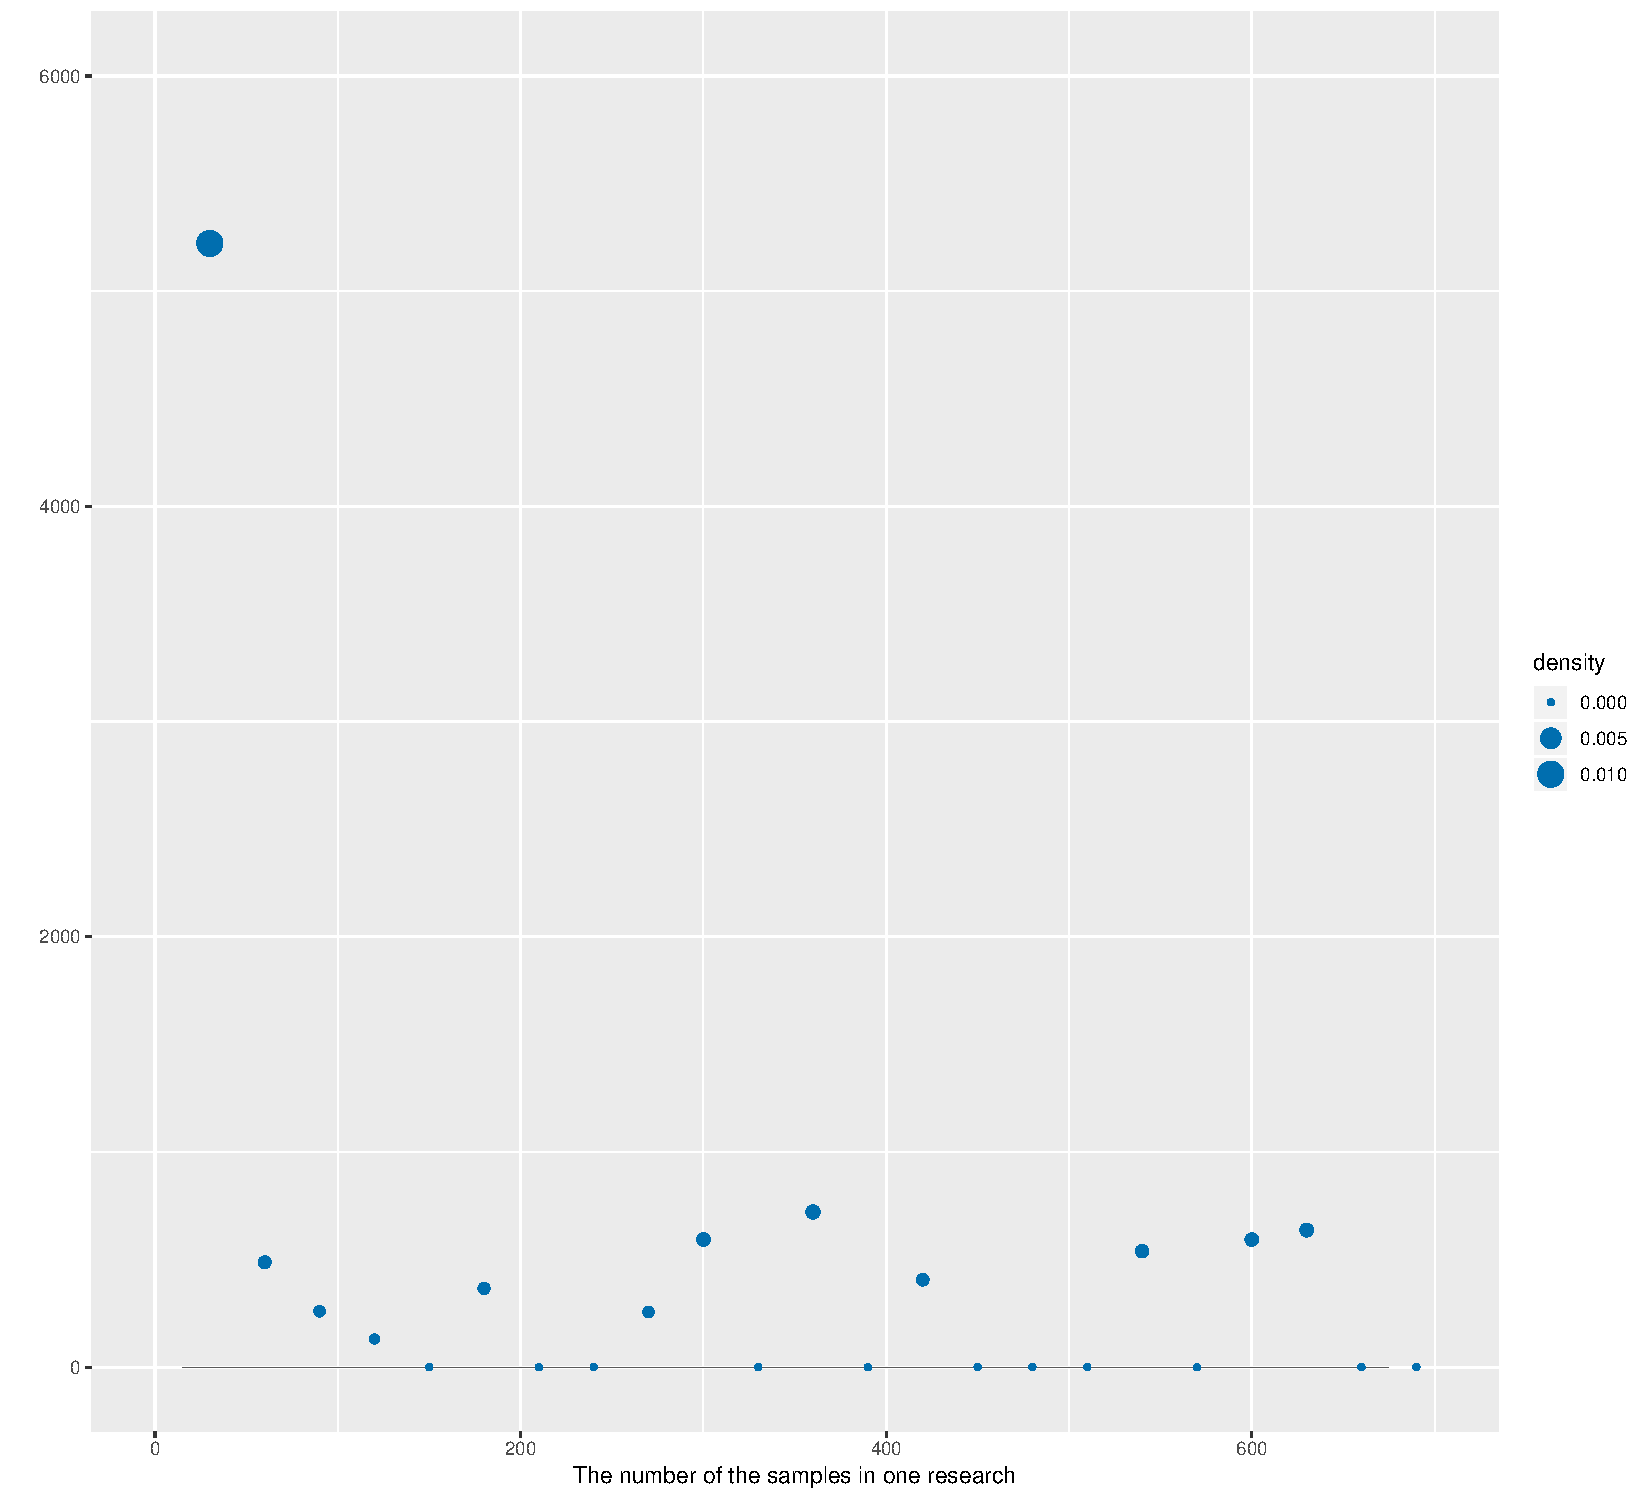
\includegraphics[width = \textwidth]{../Results/number.pdf}
		\caption{The size of samples within one research, most researches contains less than 50 samples.}
	\end{figure}

	\subsection{Comparisons in performances of models fitting in habitats}
	Overall, the performances of all the models fitting in different habitats have significant difference, the p value < 1.534e-07. Cubic model has the best fitting performance over other three Schoolfield models. Within the three forms of Schoolfield models, the Schoolfield model for high temperature has the best performance.
	
	In freshwater environments, under AIC, BIC, and AICC, the four models have different performances. All the pairwise p value < 0.01, only one p value between Schoolfield model and Schoolfield model under AICC is 0.01296. And Cubic model fits best, especially under AICC.
	
	In marine environments, only under AICC, the Cubid model has significant difference with other three Schoolfield models. Under AIC and BIC, there isn't significant difference with the four models. The reason could be penalty of the number of parameters from AICC\citep{johnson2004model}.
	
	In terrestrial environments, under AICC, the Cubid model has significant difference with other three Schoolfield models. Under AIC, the Cubic model has significant difference with the Schoolfield model for high temperature and he Schoolfield model for low temperature, the p values are < 0.009082, and < 6.75e-08, respectively. And the Schoolfield model has significant difference with the Schoolfield model for high temperature and he Schoolfield model for low temperature, as well. The p values are < 0.03602, and < 1.13e-04, respectively. Under BIC, except p value between Cubic model and he Schoolfield model is > 0.05, other p value are signigicant(p values are not shown).
	
	In a word, phenomenological model has better performance than mechanistic models. Under AICC, the weight value of three forms of the Schoolfield models are exceedingly low. It is likely that there are too many parameters\citep{johnson2004model}. With the three forms, the Schoolfield model for high temperature and he Schoolfield model for low temperature have relatively good performance in marine environments. 
	 
	
	
		\begin{figure}[H]
		\centering
		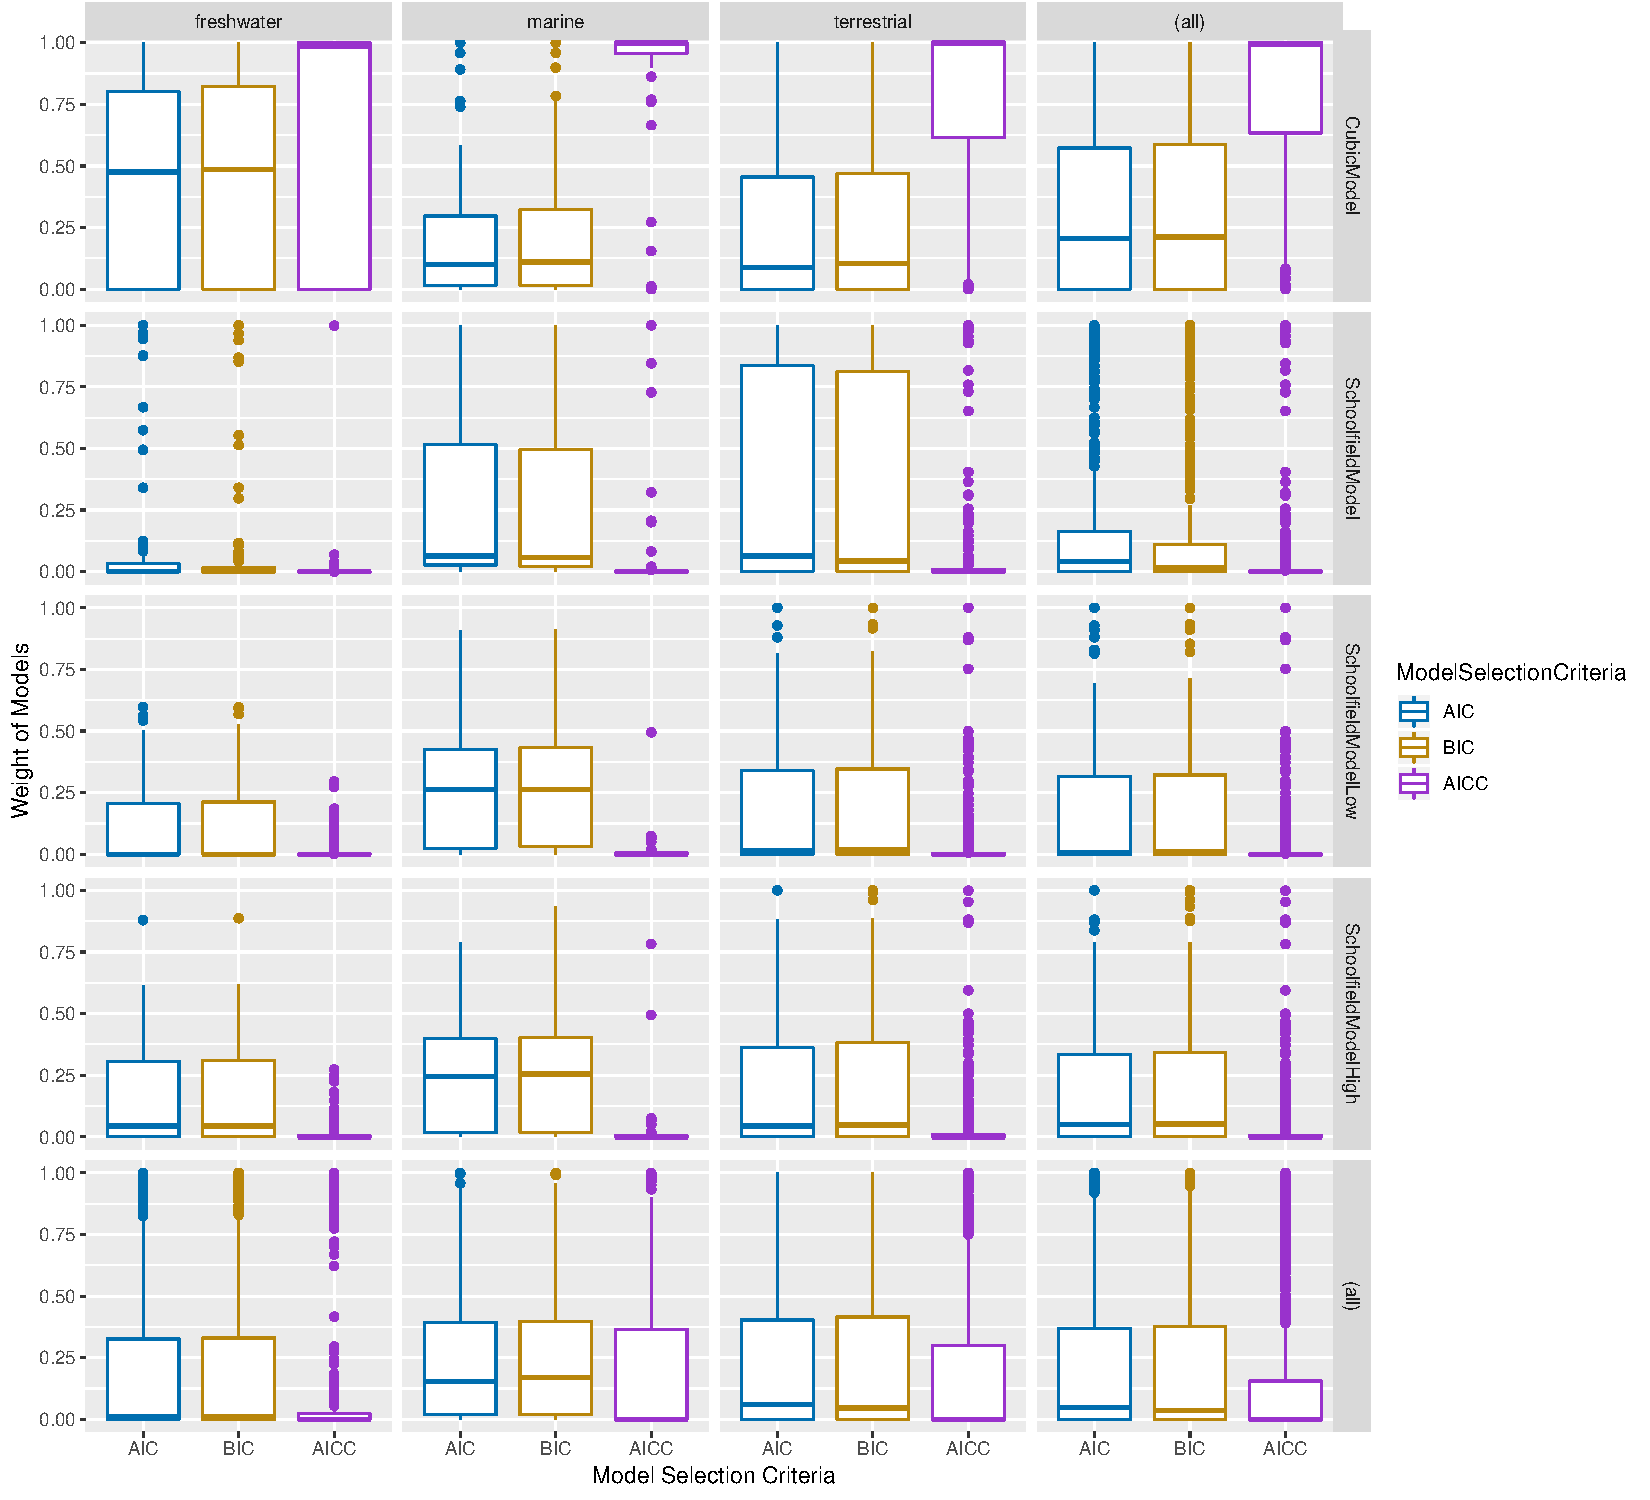
\includegraphics[width = \textwidth]{../Results/habitat.pdf}
		\caption{Comparisons in performances of models fitting in habitats. Cubic has the best performance. Under AICC, the weight value of three forms of Schoolfield model is extremely low.}
	\end{figure}
	
	\subsection{Four models fitting one research}
	The FinalID of this research is MTD5347\citep{ratkowsky2005unifying}, the species is bacterium, \textit{Escherichia.coli}, the original trait name is Square Root (Maximum Specific Growth Rate).  The reason why this plot can only show three models is that the Schoolfield model for high temperature and the Schoolfield model for low temperature are quite similar and are overlapped. 
		\begin{figure}[H]
		\centering
		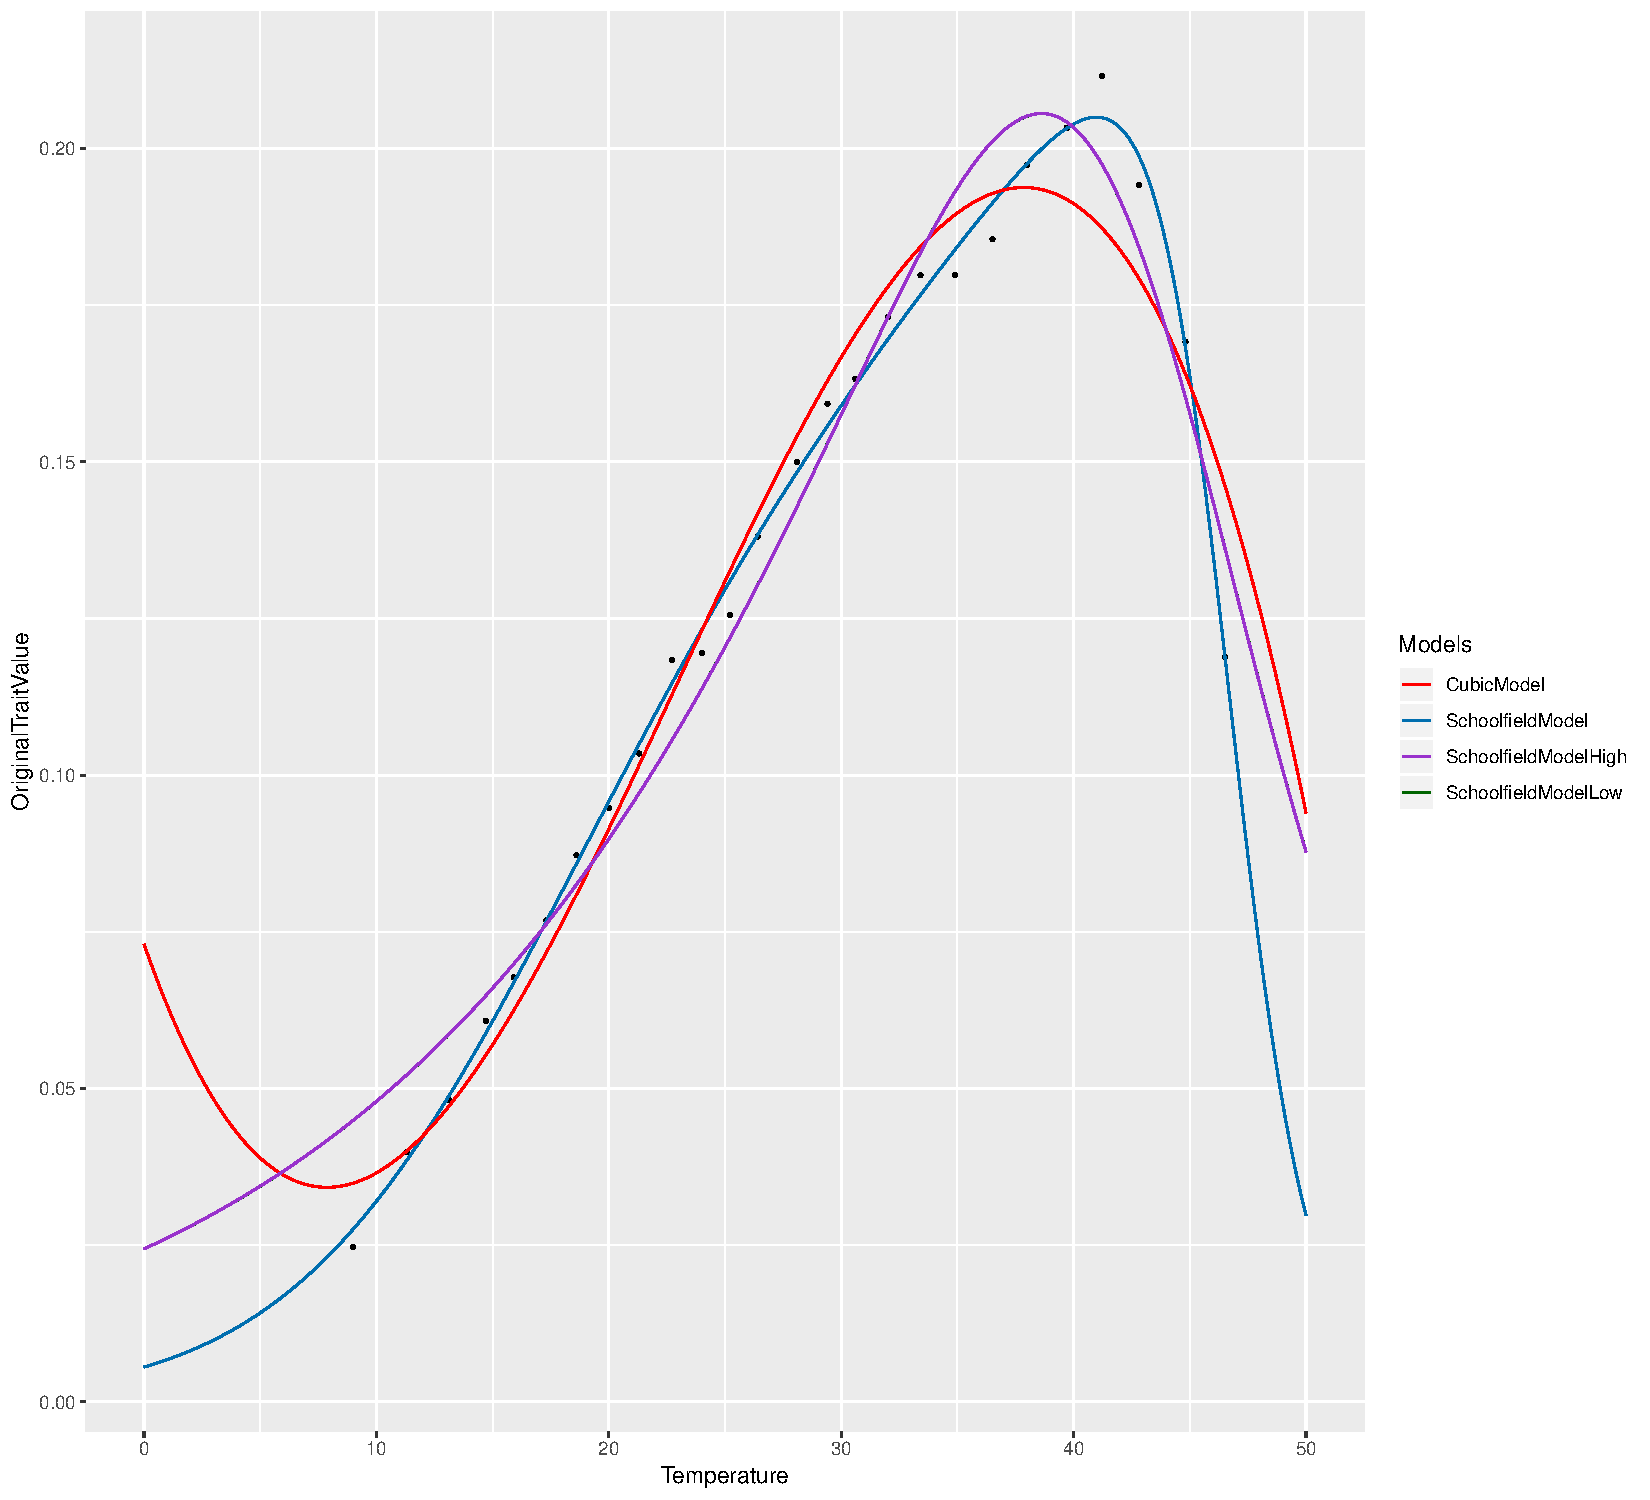
\includegraphics[width = \textwidth]{../Results/model_951.pdf}
		\caption{The four models fitted on one research. This curve shows the growth rate of \textit{Escherichia.coli}. }
	\end{figure}
	
		\section{Discussion}
		\subsection{The reason behind the different performance}
		To star with, the distince temperature ranges in different habitats is considered. For instance, under water, most organisms do not experience temperatures above 25$^\text{o}$C – 30 $^\text{o}$C, but in terrestrial environments, high tempratures of 36$^\text{o}$C - 40 $^\text{o}$C are common in summer. 
		
		However, later analysis shows the assumption is not supported. If the assumption is true, the Schoolfield model for low temperature should have much better performance than others. As shown above, that results are not drawn. Accordingly, researches on the reason are needed.
		\subsection{Limitations}
		\subsubsection{Without further mining}
		The large dataset contains many interesting contents. But this report is without further mining. For instance, many Kingdom are included. Overall, the four models have significant difference at Kingdom level, the p value is 1.55e-10. But the pairwise significant difference were not calculated. The reason has not been considered, either.
		
		\begin{figure}[H]
		\centering
		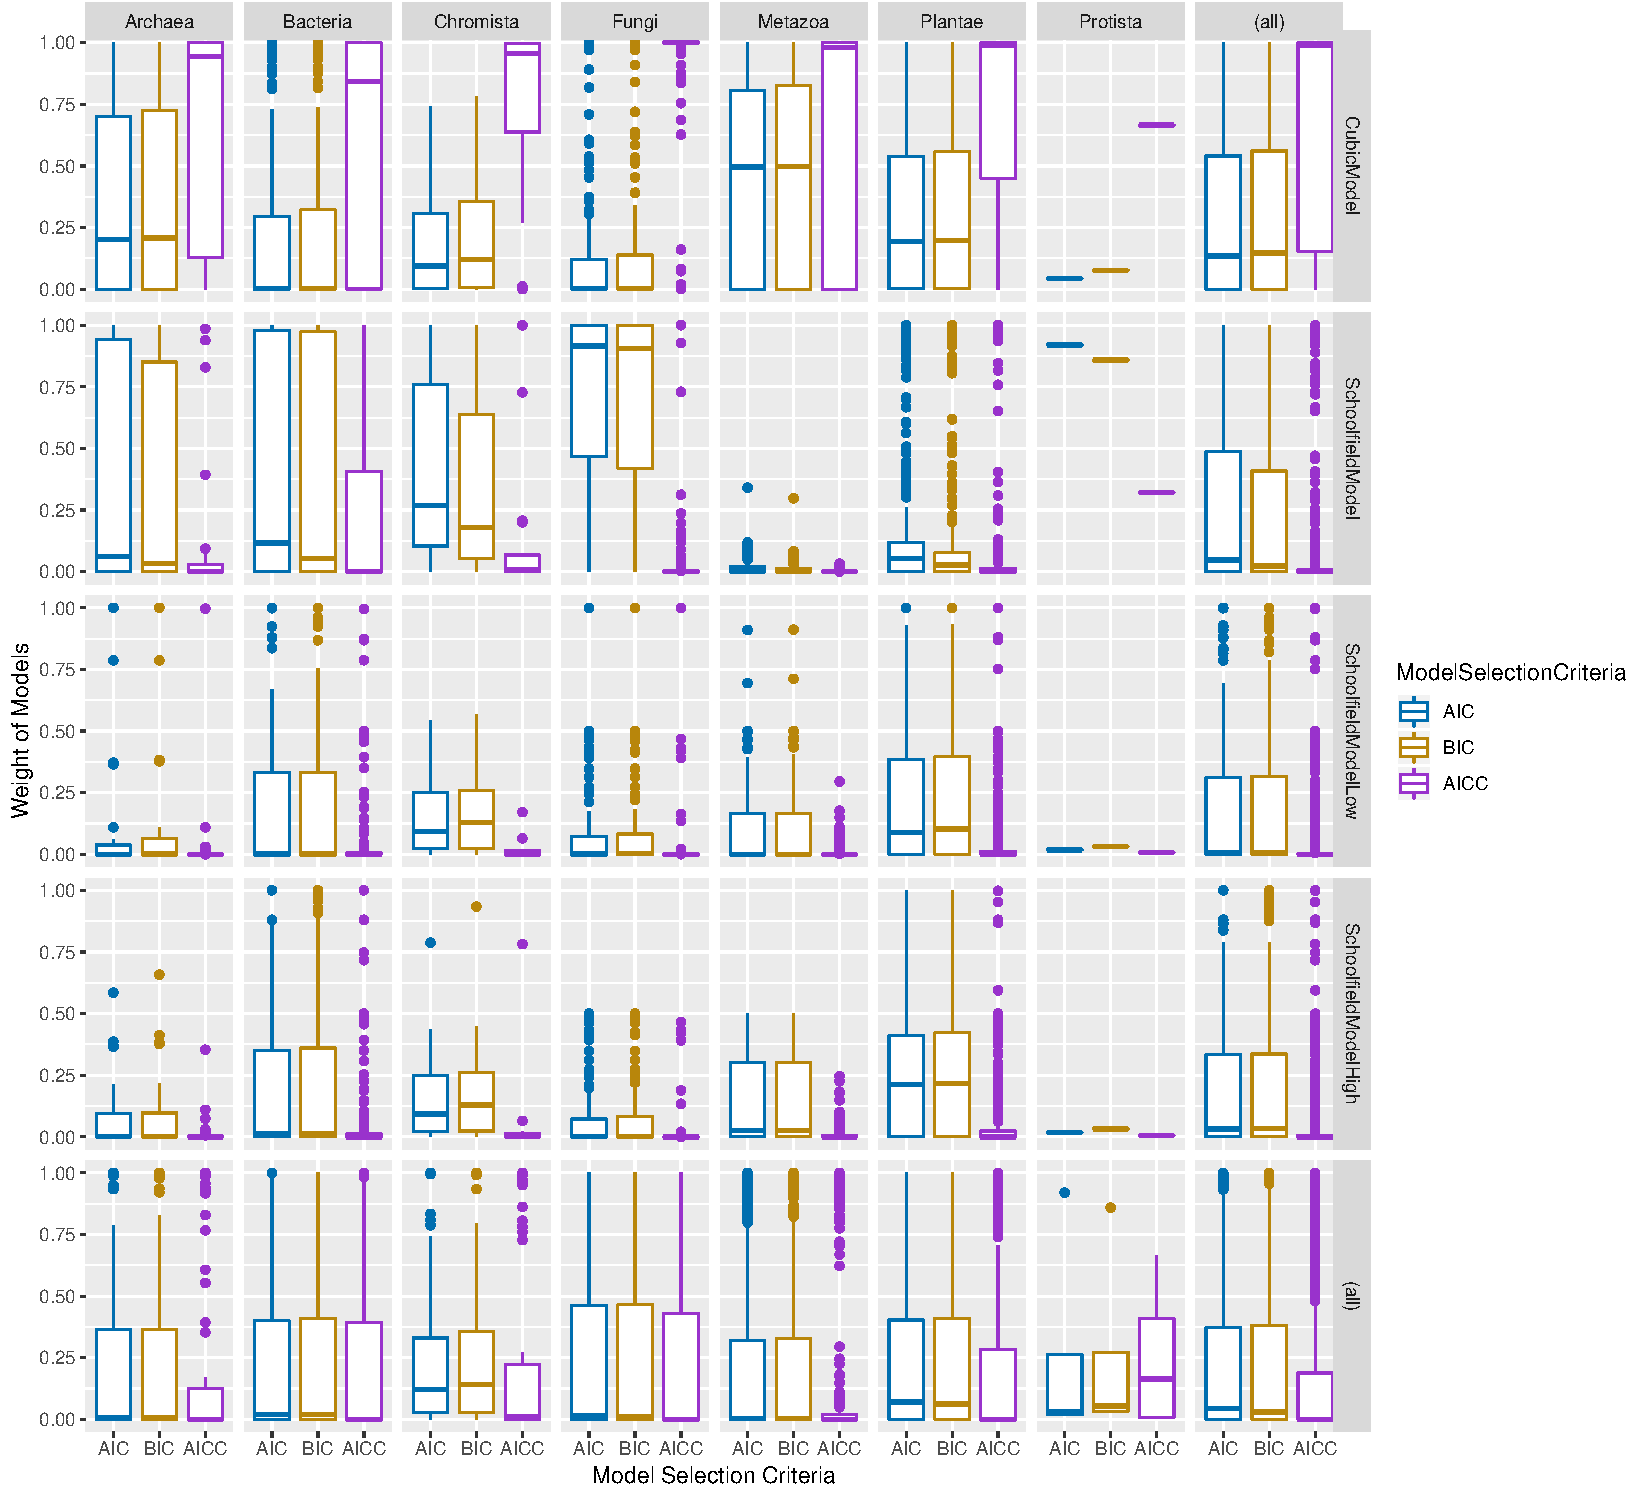
\includegraphics[width = \textwidth]{../Results/kindom.pdf}
		\caption{Comparisons in performances of models fitting in different organisms at Kingdom level.}
	    \end{figure}
	    
		\subsubsection{Without further understanding of the model selection criteria}
		The extremely low weight value of Schoolfield models is due to the penalty of the numbers of parameters from AICC. But the difference between AIC and BIC has not been discussed.
		
		\subsubsection{Visual flaw}
		Some of the figures are too complicated to add p values, and all the p values can't be shown at the figures.
		
		\section{Conclusion}
		In conclusion, phenomenological model has better performance than mechanistic models in different habitats. As for mechanistic models, in different habitats and under different model selection criteria, there is better model to choose. Researchers are supposed to choose the better models and model selection criteria carefully in terms of the specific background, habitat and so forth.
		
		We need more researches to study to mechanisms behind the metabolic reactions and propose mechanistic models with precise prediction, which is especially essential at the time when extreme climate frequent and climate change has a critical influence on agriculture, fisheries, and health.
	

	
	 




	
		
	

	
	
	
	\newpage
	\bibliographystyle{agsm}
	\bibliography{miniproject}

\end{document}